\documentclass[letterpaper, 10 pt, conference]{ieeeconf}

\IEEEoverridecommandlockouts
\overrideIEEEmargins

\usepackage{graphicx}
\usepackage{subfig}

\usepackage[tbtags]{amsmath}
\usepackage{amsfonts}

\usepackage{paralist}

\usepackage{url}

\renewcommand{\vec}[1]{\boldsymbol{#1}}
\newcommand*{\R}[1]{\mathbb{R}^{#1}}

\def\figurename{Fig.}

\begin{document}

	\title{\LARGE \bf Task-Level Teleoperated Manipulation \\ for the HRP-2Kai Humanoid Robot}

	\author{Rafael Cisneros, Shuuji Kajita, Takeshi Sakaguchi, \\
					Shin'ichiro Nakaoka, Mitsuharu Morisawa, Kenji Kaneko, Fumio Kanehiro
	\thanks{R. Cisneros, T. Sakaguchi, S. Kajita, S. Nakaoka, M. Morisawa, K. Kaneko and F. Kanehiro
					are with the National Institute of Advanced Industrial Science and Technology (AIST),
					305-8568 Tsukuba, Japan.
					{\tt\small \{~rafael.cisneros, s.kajita, sakaguchi.t,
					s.nakaoka, m.morisawa, k.kaneko, f-kanehiro~\} @aist.go.jp}}}
  
	\maketitle

	\thispagestyle{empty}
	\pagestyle{empty}

	\begin{abstract}
		This paper presents the strategy used by our team, AIST-NEDO, at the DARPA Robotics Challenge to deal
		with the designated manipulation tasks by means of a task-level teleoperation of the HRP-2Kai humanoid robot,
		considering a disaster-hit scenario that is inherently non-structured and a limited communication between the
		user and the robot.
		The strategy, based on the information provided by a laser rangefinder and a set of cameras installed
		at the head and at both hands, consisted in the alignment of 3D models representing the desired manipulation
		targets with a measured point cloud, in order to provide a reference frame to describe the manipulation motion
		required for each task.
		Each motion was carefully planned in advance by assuming minimum information of the object representing the
		manipulation target.
		In order to exemplify the before mentioned approach, two representative tasks of the DARPA Robotics Challenge
		are described, as well as the corresponding results obtained during the competition.
	\end{abstract}

	\section{Introduction and Motivation}
	\label{sec:introduction}

	Disaster response is attracting attention from the robotics research community, and even more since the
	Fukushima Daiichi nuclear power plant accident that followed the 2011 Great East Japan earthquake and tsunami.
	As a concrete materialization of this increasing interest, a challenge is proposed by the American Defense
	Advanced Research Projects Agency (DARPA) to use robots in disaster-hit facilities that were made too hazardous
	for direct human operator intervention.
	It is worth noticing that the challenge does not impose any constraint on the design of the robot, but since the
	environment (industrial ladders, doors, valves, cars) as well as the tools (levers, drills, hammers) were meant
	to comply with the human morphology, it is a natural option to develop the necessary means to make the humanoid
	robots capable of performing inspection and disaster recovering actions inside a non-structured environment
	\cite{Bouyarmane}.
	
	This environment can be considered to be ``kind of'' known in the sense that we know which actions
	are required in advance and that we have a rough idea of its spatial distribution,
	maybe altered due to the disaster itself.
	Then, only very limited assumptions about the structure of the environment can be made beforehand,
	in contrast to structured scenarios where semantic knowledge of their structure can be leveraged
	for highly autonomous robots operating in them~\cite{Kohlbrecher}.
	
	It is also mandatory to consider that within a disaster-hit facility it is not possible to rely on a stable,
	wide bandwidth wireless communication system with the robot.
	The signal may be degraded and blackouts may occur frequently.
	Then, it is not feasible to consider a purely teleoperated robot.
	First, because of the high dimensionality of its control system, and second because the capabilities of
	the robot and the operator should include near real-time feedback without disruptions in the communications
	as well as transmission of large amounts of data to the operator.
	On the other hand, a fully autonomous robot navigating and interacting in an unconstrained environment
	should include extensive databases of information about possible objects of interest to be found,
	highly efficient grasping algorithms and the ability to react to unforeseen situations,
	which are still unsolved problems~\cite{Romay}.
	A feasible alternative is the development of supervised semi-autonomous high Degrees-Of-Freedom (DOF)
	robotic systems; that is, task-level teleoperated systems in which the operator cognitive burden is
	minimized by lowering the control space dimensionality~\cite{Katyal}, such that these operators function
	as supervisors setting high level goals, assisting the robot with complex perception tasks, directly
	changing robot parameters to improve its performance and making decisions when facing unexpected
	situations~\cite{Kohlbrecher}.
	
	\section{Related Work}
	\label{sec:related_work}	
	
	\section{HRP-2Kai humanoid robot}
	\label{sec:hrp2kai}
	
	HRP-2Kai stands for Humanoid Robotics Platform no.~2 Improved (Kai means improvement in Japanese).
	This humanoid was developed in phase two of the Japanese national project HRP
	(Humanoid Robotics Project) and was recently improved to be able to cope with disaster response
	tasks~\cite{Kaneko}.
	
	This robot, depicted in \figurename~\ref{fig:HRP2Kai-robot}, has the kinematic structure shown
	in \figurename~\ref{fig:HRP2Kai-structure}.
	As seen in this diagram, the robot has 32 dof:
	6 at each leg, 2 at the waist, two at the head, 7 at each arm and 1 at each hand.
	This robot features a set of exteroceptive sensors that are actively used during the manipulation
	tasks: a 3D scanner system built in its head and four cameras, placed at the head, at the back and
	at each hand.
	The 3D scanner system was implemented with a Laser Range Finder (LRF) synchronized with the head
	pitch joint, as shown in \figurename~\ref{fig:3DScanner}.
	The hand camera is mounted in each hand as shown in \figurename~\ref{fig:Hand}, together with a
	LED light and a laser.
	It is worth to mention that this camera is not lined up with the longitudinal axis at the center
	of the hand.
	
	\begin{figure}[t]
		\begin{center}
			\subfloat[Actual robot.]{\label{fig:HRP2Kai-robot}
				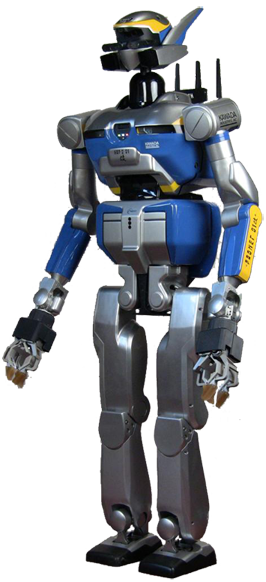
\includegraphics[height = 4.3cm]{img/HRP2Kai-robot}}
			\hspace{1cm}
			\subfloat[Structure.]{\label{fig:HRP2Kai-structure}
				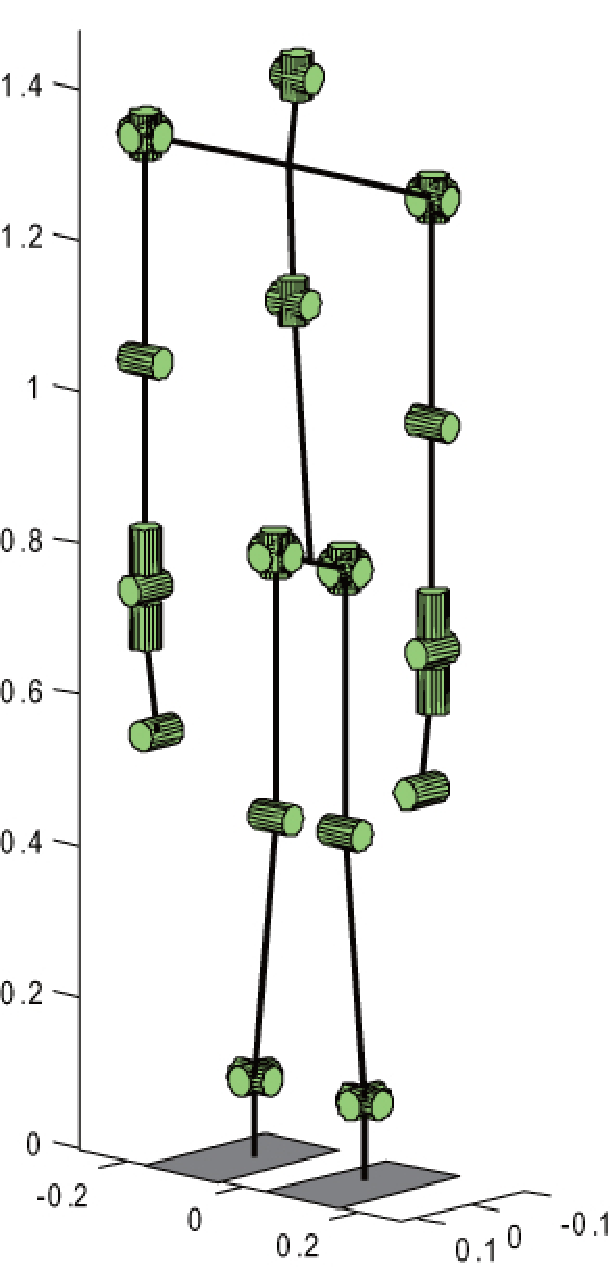
\includegraphics[height = 4.3cm]{img/HRP2Kai-structure}}
		\end{center}
		\caption{HRP-2 Kai humanoid robot.}
		\label{fig:HRP2Kai}
	\end{figure}
	
	\begin{figure}[b]
		\begin{center}
			\subfloat[3D scanner and head camera.]{\label{fig:3DScanner}
				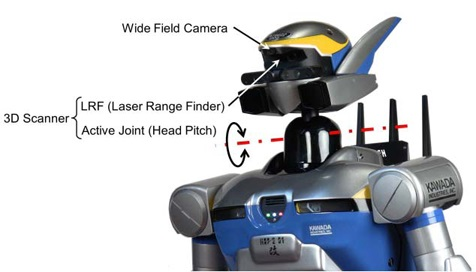
\includegraphics[height = 3cm]{img/3DScanner}}
			\hspace{0.25cm}
			\subfloat[Left hand camera.]{\label{fig:Hand}
				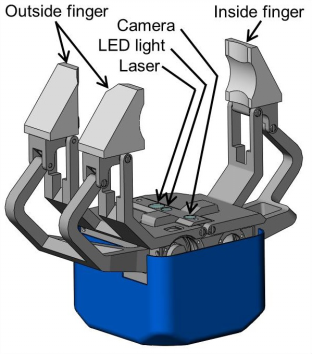
\includegraphics[height = 3cm]{img/Hand}}
		\end{center}
		\caption{Exteroceptive sensors of HRP-2 Kai~\cite{Kaneko}.}
		\label{fig:HRP2Kai}
	\end{figure}
	
	\section{Graphical User Interface for Teleoperation}
	\label{sec:teleoperation_gui}
	
	The Graphical User Interface (GUI) used for the teleoperation of HRP-2Kai was implemented
	in Choreonoid, an integrated robotics GUI environment~\cite{Choreonoid}~\cite{Nakaoka_Choreonoid}.
	A snapshot of this GUI is shown in \figurename~\ref{fig:Choreonoid3}.
	
	As can be seen, the teleoperation interface features several windows, each one of them
	corresponding to
	%
	\begin{inparaenum}[(1)]
		\item the scene view,
		\item the task sequencer,
		\item the head camera,
		\item the right hand camera,
		\item the left hand camera,
		\item the item view, and
		\item the property view.
	\end{inparaenum}
		
	\begin{figure}[t]
		\centering
		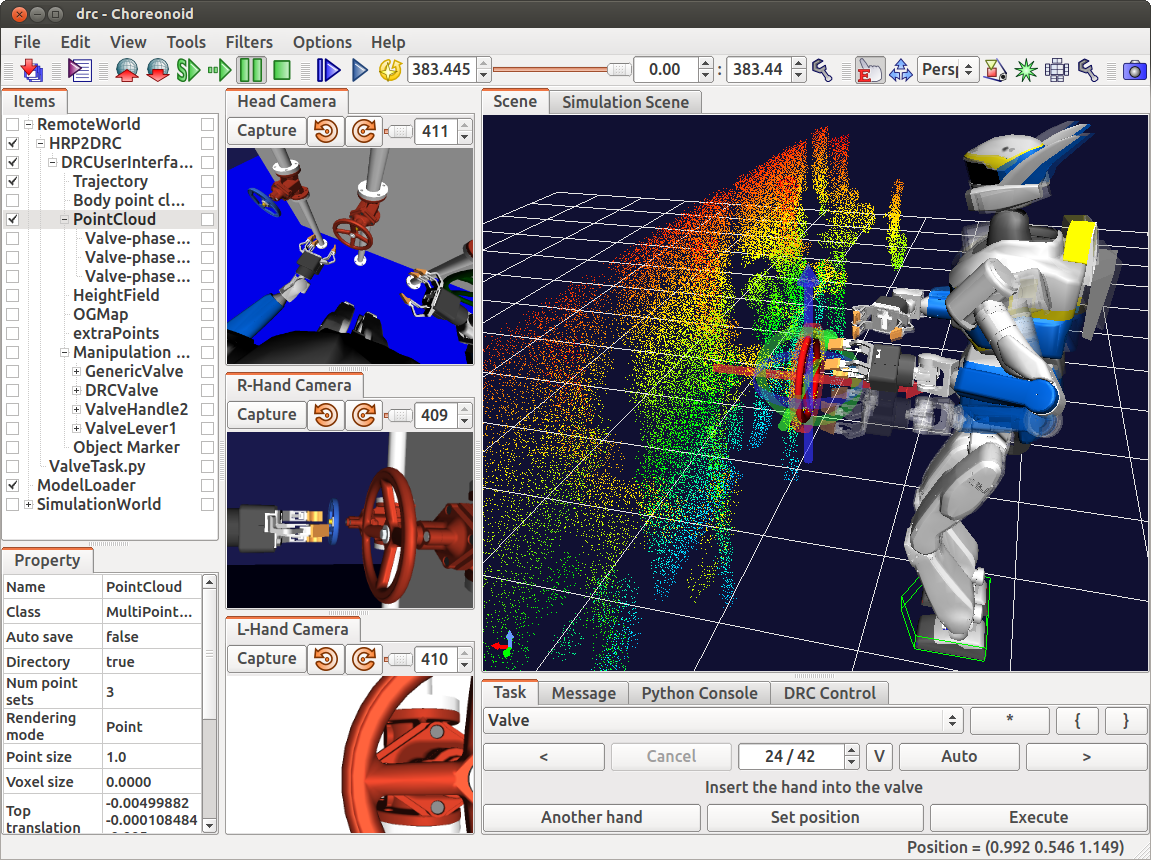
\includegraphics[height = 5.85cm]{img/Choreonoid3}
		\caption{Teleoperation interface in Choreonoid~\cite{Nakaoka_Humanoids}.}
		\label{fig:Choreonoid3}
	\end{figure}
	
	The scene view is used to teleoperate the robot through the direct control of a 3D model
	showing the robot's current configuration, as well as the planned motion represented by
	one (or several) translucent version(s) of the robot, one per each key configuration.
	The \emph{point cloud} of data corresponding to the measured points on the surface of the
	objects in the environment is captured by the 3D scanner and presented also in the scene view.
	From this information it is possible to extract the \emph{height field} of the floor,
	used by the walking control system to achieve a stable gait over uneven terrain~\cite{Morisawa},
	as well as to detect obstacles and objects of interest in the environment in order to perform
	a proper whole-body collision-free posture planning, as required by the manipulation
	task~\cite{Kanoun}.
	
	The object that is the target of the manipulation task can be identified in the point cloud
	by overlapping a simplified 3D model of it, as shown in \figurename~\ref{fig:Choreonoid3}.
	This model, referred as \emph{Manipulation Marker}, provide a reference frame with respect
	to which the manipulation task can be described once it is aligned with the corresponding
	points.
	This alignment can be done manually by using a set of arrows and rings provided by the interface
	to translate and rotate the marker, or automatically with the aid of a built-in function included
	in the Point Cloud Library (PCL), used by Choreonoid.
	
	The manipulation motion is specified by providing the pose (position and orientation)
	of the hands of the robot, and calculated by solving the whole-body inverse kinematics
	problem~\cite{Kanoun}.
	This motion can be either planned in advance or manually changed during the execution of the task
	by using \emph{Hand Markers} (3D models of the hands that can also be translated and rotated).
	
	The \emph{task sequencer} is provided by the interface to execute each manipulation
	task step by step according to its state, such that the complex perception and supervision
	be entrusted to the operator.
	
	On every step of the task, the robot is commanded to go to a predefined stance and/or to reach a
	predefined posture, both of them relative to a previously identified target.
	Then, the robot autonomously generates the required motion to accomplish the desired configuration,
	avoiding obstacles represented by the point cloud and maintaining its dynamic stability.
	This approach makes it possible to have an ergonomic operator-robot interaction. 
	
	Finally, the interface also provides the image captured by every camera, as well as additional information.
	For example, the item window enlists the components required by Choreonoid to implement the teleoperation
	interface, together with their configuration parameters: their properties.
	
	By using this interface we implemented all the manipulation tasks required during the
	DARPA Robotics Challenge:
	%
	\begin{inparaenum}[(1)]
		\item opening a door,
		\item turning a valve,
		\item cutting a wall with a drill, and
		\item a surprise task which consisted in opening a box and pushing a button (rehersal day),
					pulling down a lever (first day of the competition) or
					pulling a plug out of a socket and inserting it into another one (second day of the competition).
	\end{inparaenum}
	%
	Given that the approach to implement each one of them was similar,
	we will only explain two representative ones:
	the door task and the plug task.
	
	\section{Door task}
	\label{sub:door}

\subsection{Outline of the door task}
%
At the DRC Finals, the door task was specially important because without passing through it,
the robot wouldn't be able to perform the five remaining tasks
(valve, wall, surprise, debris or terrain, and stairs).
   
In general, we can divide the execution of the door task into the following phases:
%
\begin{enumerate}
	\item Walking to the front of the door.
	\item Grasping the door lever.
	\item Turning the lever and opening the door.
	\item Walking through the door.
\end{enumerate}
%

%In the DRC Finals, it was announced that the door will be 
%
%\begin{itemize}
%\item push open style,
%\item with lever type door lever, and
%\item without door closer.
%\end{itemize}

At the end of the second phase, the robot ends up in a standing configuration with a hand grasping
the door lever.
Let us call this the {\it open-door pose} as illustrated in \figurename~\ref{fig:door_approaching_config}.
In our approach, we determine a specific standing stance and a wrist attitude with respect to 
the door lever as shown in the figure.
In this way, the remaining phases 3) and 4) start from the same configuration;
thus we can use a pre-programmed sequence for operating the door and passing through it.
Even if we face variations of the door's geometry,
they can be handled by means of a minimum modifications.

\begin{figure}[t]
  \centering
  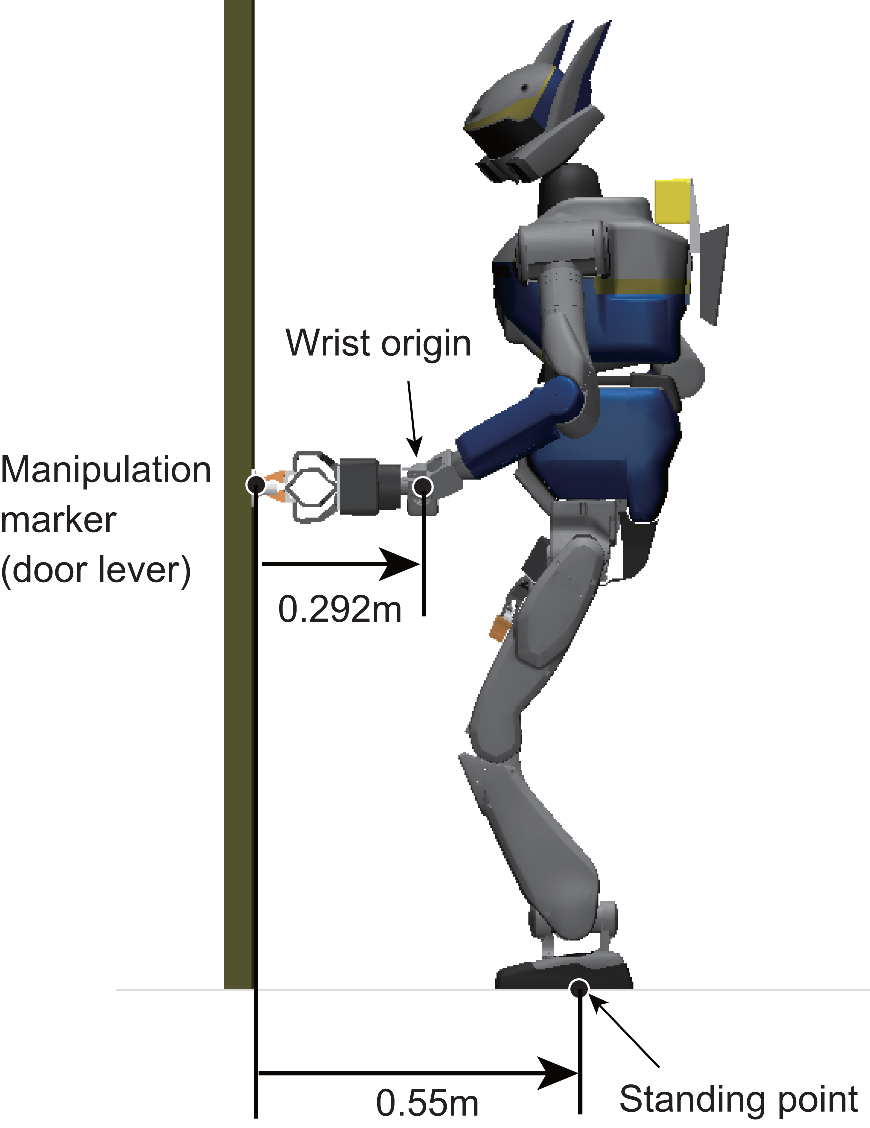
\includegraphics[width = 6.25cm]{img/door_approaching_config}
  \caption{Open-door pose}
  \label{fig:door_approaching_config}
\end{figure}

%From Step1 to Step2, we control our robot to realize the door approaching pose.
%To realize a reliable door passing, we pre-determined
%a robot pose grasping the door lever.
%Let us call it as {\it door approaching pose} which specifies the
%wrist point and the standing point with respect to the door lever

%The door lever operation (Step3) and the door passing through (Step4) always start
%from this fixed configuration. This means we can use a programmed sequence or its minimum
%modification at the door task.  

In the following subsections, we explain in detail phases 1) and 2); that is,
the way to control the robot to achieve the open-door pose by using sensor information
and teleoperation.
Phases 3) and 4) can be easily implemented. 
Especially at the DRC Finals, once the door had been opened wide enough, it ended up opening
completely by means of gravity and remaining open, since the door hinge was inclined 2.6 degrees
away from the vertical.
This helped the robots to walk through the door without worrying about any collision with
the opened door panel, which would eventually hit the robot by means of the action of the wind if the door hinge 
was vertical. 

\subsection{Walking to the front of the door}
%
To navigate the robot to the pose specified in \figurename~\ref{fig:door_approaching_config},
we used the point cloud data measured by the LRF. 
We took a two-step manual operation to identify the door orientation and the position of the
door lever as illustrated in \figurename~\ref{fig:door_manip_markers}.

First, the operator specifies a point on the left edge of the door panel
(\figurename~\ref{fig:door_manip_markers}(a) the `x' mark pointed by the arrow).
By applying the least square method to the portion of the point cloud located at the right of
the specified point, we can calculate the orientation of the door panel.
The result is shown by the {\it door marker}, a gray rectangle in
\figurename~\ref{fig:door_manip_markers}(b).
It covers a part of the door panel and we can interactively manipulate it on the point cloud GUI.
By adjusting the door marker, we can mask the points of the door panel and extract the points of
the door lever as shown in \figurename~\ref{fig:door_manip_markers}(c).
%Since the door lever is relatively small with respect to the point cloud resolution,
%it contains only 10 to 20 points which makes conventional model fitting very difficult.
%Thanks to the robustness of the human perception, 
In this way, we can confidently mark the rotation center of the lever (pointed by the arrow).
\figurename~\ref{fig:door_manip_markers}(d) shows the manipulation marker for the door lever
placed on the point cloud.
Its position and orientation are used to navigate the robot to the desired pose for opening
the door.

\begin{figure}[t]
  \centering
  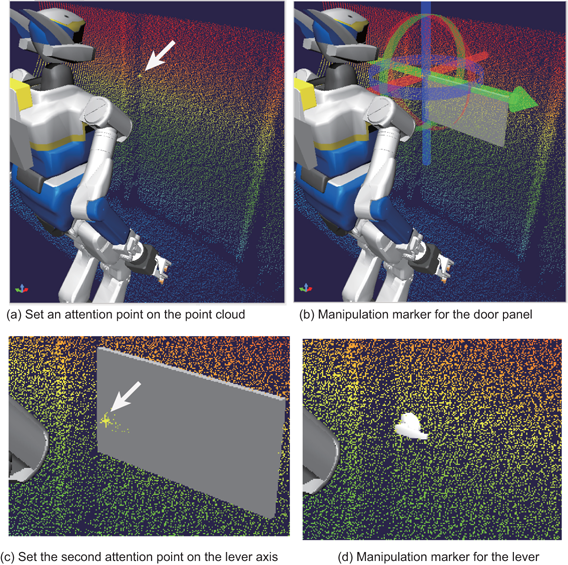
\includegraphics[width = 8cm]{img/door_manipulation_markers}
  \caption{Detection of the door lever in the control window}
  \label{fig:door_manip_markers}
\end{figure}

\subsection{Grasping the door lever}
%
Now the robot is standing on a good place to grasp the door lever.
%By the method of previous subsection, we can expect our robot is standing in front of the door
%aligned to its surface normal with desired distance.
Instead of grasping the door lever directly, we move the robot hand to an {\it approach point},
which is placed at a certain distance (0.13m) from the lever. 
This is because the hand position may not be accurate enough due to the LRF measurement noise,
calibration error, and slip occurring while walking.

Figure \ref{fig:door_lever_grasp}(a) shows the robot at the open-door pose and its hand at the
approach point (right window) in Choreonoid simulator.
The left window shows the simulated view of the left hand camera.
Both images show that the left hand is not appropriate to grasp the door lever (too left).
Note that during the real robot control, only the camera view is available. 

The operator can manually adjust the hand position by using some GUI buttons: 
{\it Left}, {\it Right}, {\it Down}, and {\it Up}, as seen in the left bottom window.
In this case, the operator can adjust the hand position by hitting {\it Right} button
several times.
Figure \ref{fig:door_lever_grasp}(b) shows the adjusted hand position to grasp the lever.

Figure \ref{fig:door_lever_grasp}(c) shows the final state getting a good grasp of the door lever.
From this moment, the point cloud based manipulation marker is no longer used.
For example, the rotation center of the lever is determined using the hand position calculated from
the internal sensors (joint encoders and posture sensors). 
%By hitting the button 'OK', the robot move the left hand forward until it contacts the door surface (we specified a sleshold of 5N to detect the contact).  The hand is in contact with appropriate position to grasp the door lever in \figurename~\ref{fig:door_lever_grasp}(c).
%
\begin{figure}[t]
  \centering
  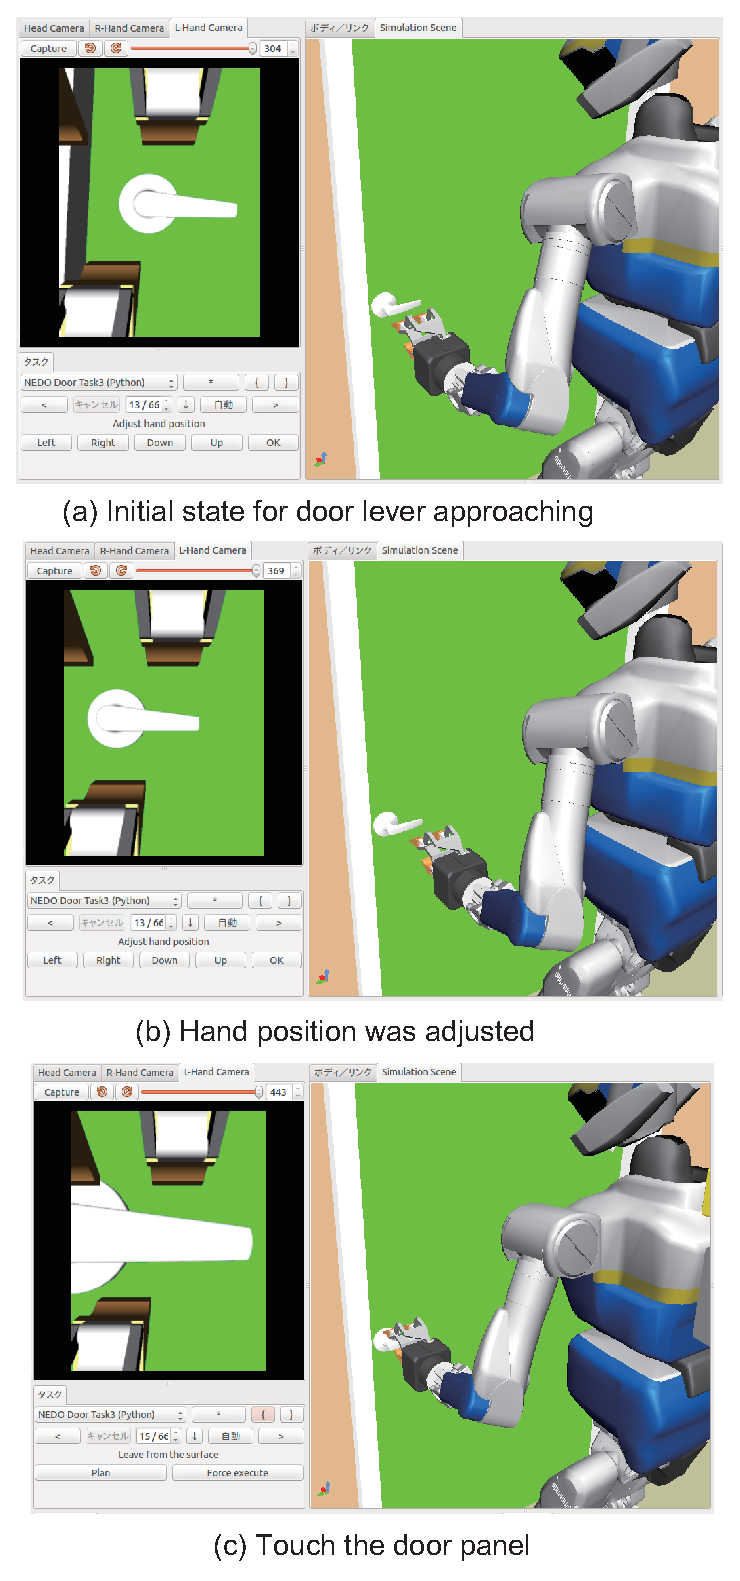
\includegraphics[width = 7.5cm]{img/approach_door_lever}
  \caption{Approach for grasping the door lever}
  \label{fig:door_lever_grasp}
\end{figure}

%\begin{figure}[t]
%  \centering
%  \includegraphics[width = 7.5cm]{img/open_the_door}
%  \caption{Door opening}
%  \label{fig:door_opening}
%\end{figure}

\subsection{Result at the DRC Finals}
%
At the DRC Finals 2015, HRP-2Kai cleared the door task at the rehearsal on June 4 and during
the challenge on June 6.
\figurename~\ref{fig:drc_door_aist_day2} shows the robot (a) while scanning with the LRF to
obtain a point cloud, (b) walking to the the open-door pose, (c) grasping the door lever,
and (d) opening the door successfully.
The robot spent 5 minutes and 21 seconds from the LRF scanning to fully pass the door.
%
\begin{figure}[t]
  \centering
  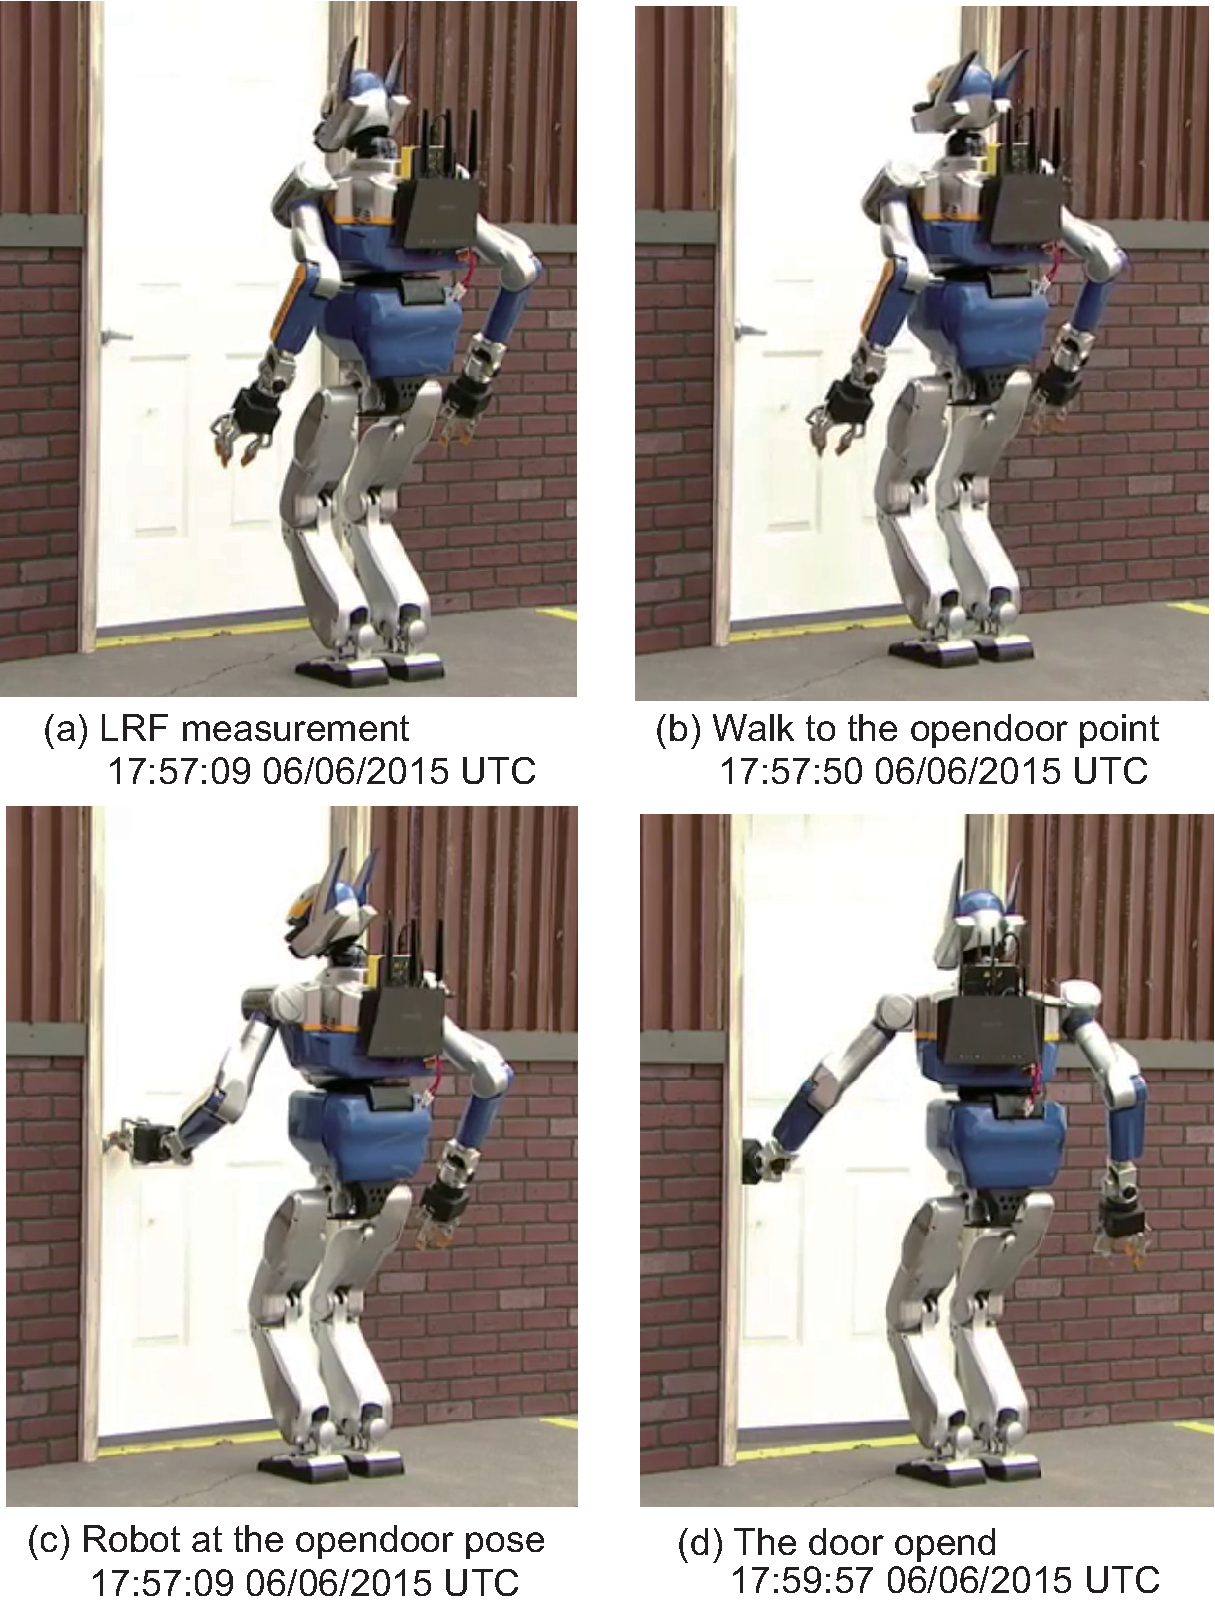
\includegraphics[width = 7.5cm]{img/drc_door_aist_day2}
  \caption{Door task at DRC Finals on June 6}
  \label{fig:drc_door_aist_day2}
\end{figure}

During the challenge on June 5, HRP-2Kai failed to operate the door lever at first,
requiring a second attempt to grasp it again, which was done by manual teleoperation.
During this operation, we experienced a low level control system crash, and the robot
fell down (\figurename~\ref{fig:drc_door_aist_day1}).
Since the computer stopped working and the hardware was damaged, we had to abort the
challenge for that day. 
%
\begin{figure}[t]
  \centering
  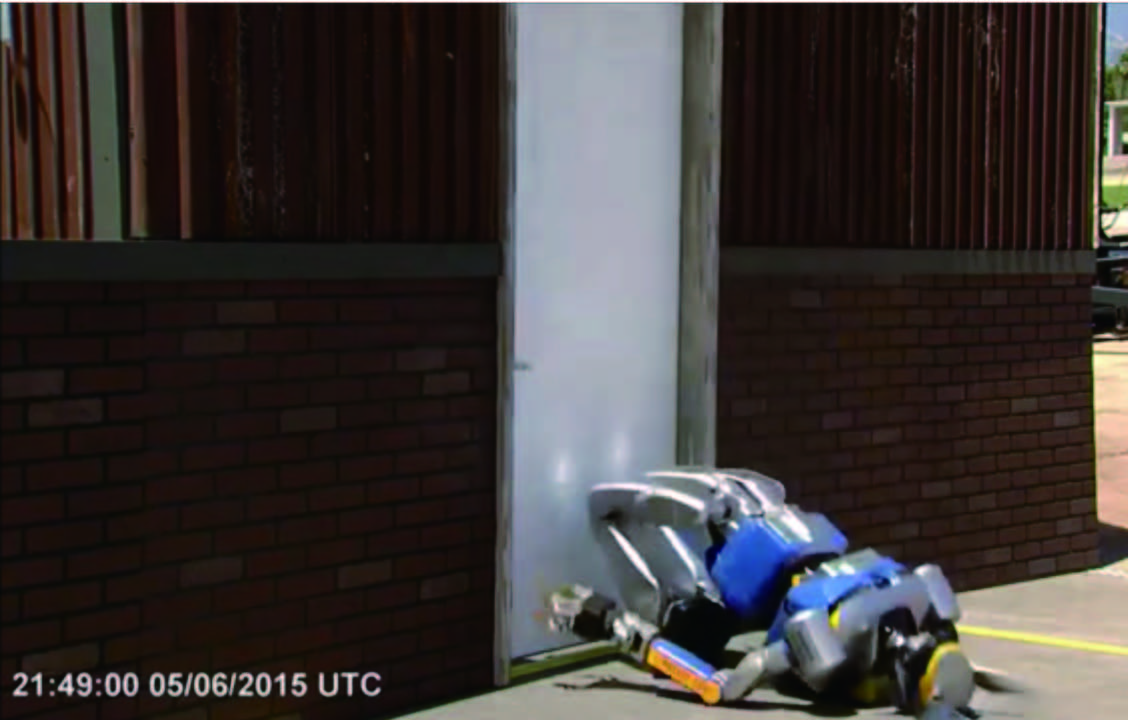
\includegraphics[width = 7.5cm]{img/drc_door_aist_day1}
  \caption{Control system crash at DRC Finals on June 5}
  \label{fig:drc_door_aist_day1}
\end{figure}

The robot failed to operate the lever because the doors in DRC Finals had different
latch properties, as shown in Table~\ref{tbl:door_latch}.
On day 1, we hard-corded the latch rotation angle as 30 degrees,
which worked at the rehearsal.
Of course, such implementation is not acceptable for the actual disaster response robots.
%
\begin{table}[htb]
\caption{Door latch properties at DRC finals} \label{tbl:door_latch}
\begin{tabular}{lclc}
\hline
Course & Latch release angle & Date & Door task result  \\ 
\hline
Green & 30 deg & June 4 (rehearsal) & Success  \\
Yellow & 70 deg & June 5 (day 1) & Fail \\
Blue &  50 deg & June 6 (day 2)  & Success \\
\hline
\end{tabular}
\end{table}


	
	\section{Pulling and inserting a plug}
	\label{sec:plug}
	
	One of the surprise tasks at the DARPA Robotics Challenge consisted of pulling out a plug
	from one socket and putting it back into another socket, in a set-up like the one shown in
	\figurename~\ref{fig:Sockets-Plug}.
	
	\begin{figure}[b]
		\centering
		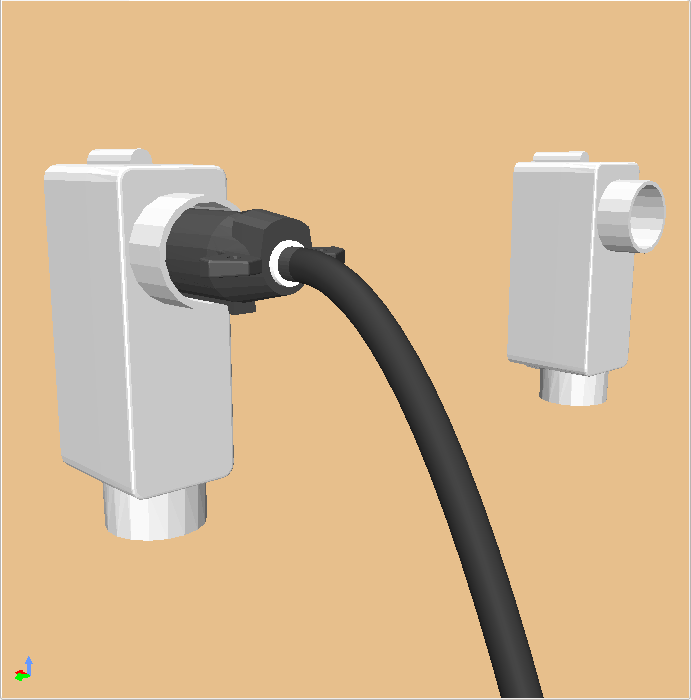
\includegraphics[height = 4cm]{img/Sockets-Plug}
		\caption{Plug Task.}
		\label{fig:Sockets-Plug}
	\end{figure}
	
	\subsection{Detection of the socket and plug}
		
		In order to perform this task it is first necessary to identify the plug and the socket where
		it is originally inserted, by placing the corresponding Manipulation Marker within the poing cloud.
		The reason to identify both objects instead of just the plug is because almost half of it
		is not visible as it is inside of the socket, making it too difficult just to match the plug,
		given the low density of points belonging to it due to its small size.
		
		By using a PCL's built in function it is possible to detect all the planes in the scene,
		one of them being the wall where the sockets are installed.
		Then, given that the front face of the sockets is parallel to this wall, it is possible
		to use the corresponding plane equation to calculate the socket's orientation with respect to
		the robot, in such a way that the plug is directed towards it.
		Having done this, one point belonging to the plug can be manually selected in order to compute
		an approximate initial position for the Manipulation Marker representing the socket and the plug.
		This one is later refined, after the robot has arrived to the desired stance and the point cloud
		has been adjusted by using the robot's hands as a reference, as seen in
		\figurename~\ref{fig:SocketPlugMarker} (and explained in Subsection~\ref{sub:uncertainties}).
		
		\begin{figure}[t]
			\centering
			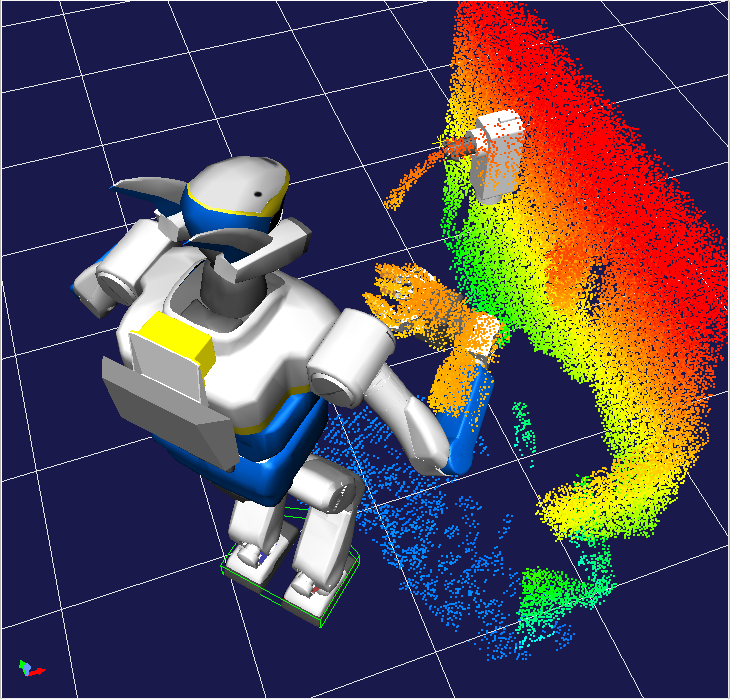
\includegraphics[height = 5cm]{img/SocketPlugMarker}
			\caption{Detection of the socket and the plug.}
			\label{fig:SocketPlugMarker}
		\end{figure}
		
	\subsection{Grasping the plug}
		
		Having detected an approximate attitude for the socket, the robot first approaches the plug
		with one hand while aligning the camera installed at the other hand with the axis of the plug.
		This is to be able to make slight adjustments of the grasping hand by using visual feedback.
		
		The size of the visible part of the plug is not that big compared to the hand of the robot,
		and because of that the tolerance for	grasping the plug is minimum.
		Then, it is required to grasp the plug at the point in which the medial side of the hand
		touches the cylindrical shaped part of the socket.
		This can be done by reducing the angle of the gripper and then, by moving the hand along the
		axis of the plug until sensing 30 N of force (enough for considering that it arrived to the socket).
		This configuration of the robot just before moving the hand towards to the socket is depicted in
		\figurename~\ref{fig:PreCloseHand}.
		
		\begin{figure}[t]
			\centering
			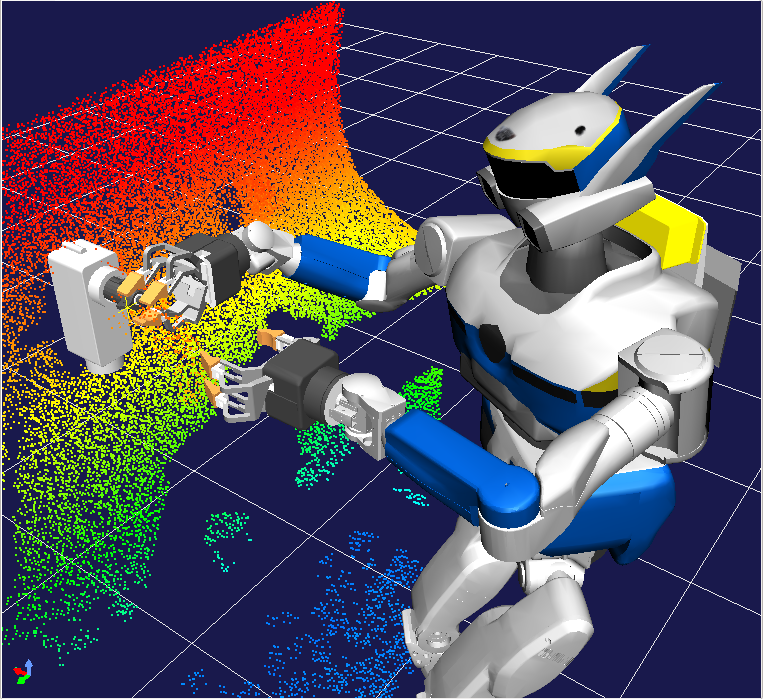
\includegraphics[height = 5cm]{img/PreCloseHand}
			\caption{Configuration of the robot before grasping the plug.}
			\label{fig:PreCloseHand}
		\end{figure}
		
		This strategy is very effective (when adjusted properly) as the grasp can be done every time at the
		desired point even in the presence of uncertainties, as shown in the dynamical simulation depicted
		in \figurename~\ref{fig:GraspPlug}.
		
		\begin{figure}[b]
			\centering
			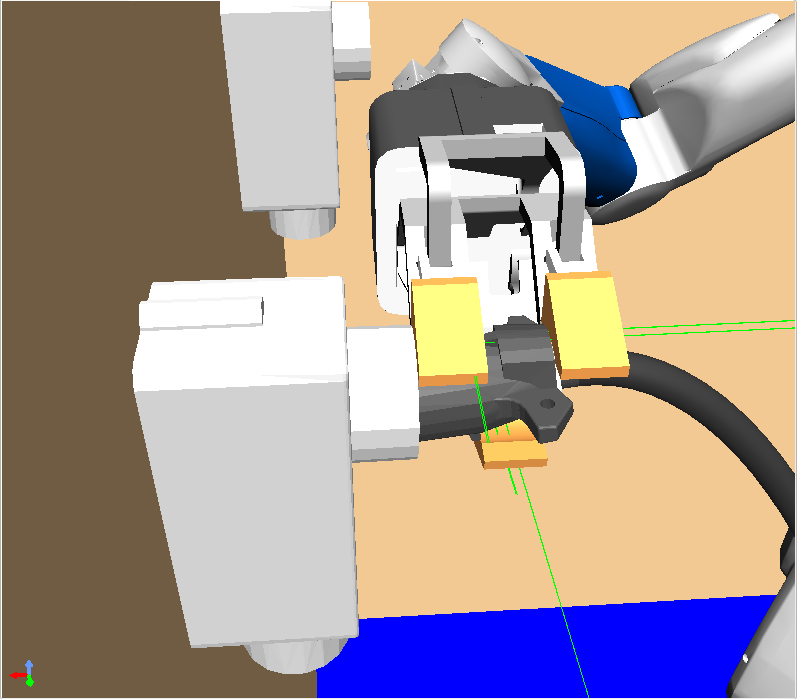
\includegraphics[height = 5cm]{img/GraspPlug}
			\caption{The plug being effectively grasped at the desired point.}
			\label{fig:GraspPlug}
		\end{figure}
		
	\subsection{Pulling and adjusting the plug}
		
		After grasping the plug, the robot pulls the plug.
		Due to the balancing process this motion may not be performed exactly along the axis of the plug,
		and it may hit the inner walls of the socket, modifying the planned relative attitude between the
		plug and the hand.
		
		For this reason, before inserting the plug into the other socket, the robot first brings the plug
		in front of its chest, takes an updated point cloud, and uses the camera placed at the head and
		at the other hand to look at the plug from two perpendicular directions, as seen in
		\figurename~\ref{fig:WatchPlug}.
		By using this information it is possible to fix the actual attitude of the plug with respect to
		the hand.
		
		\begin{figure}[t]
			\centering
			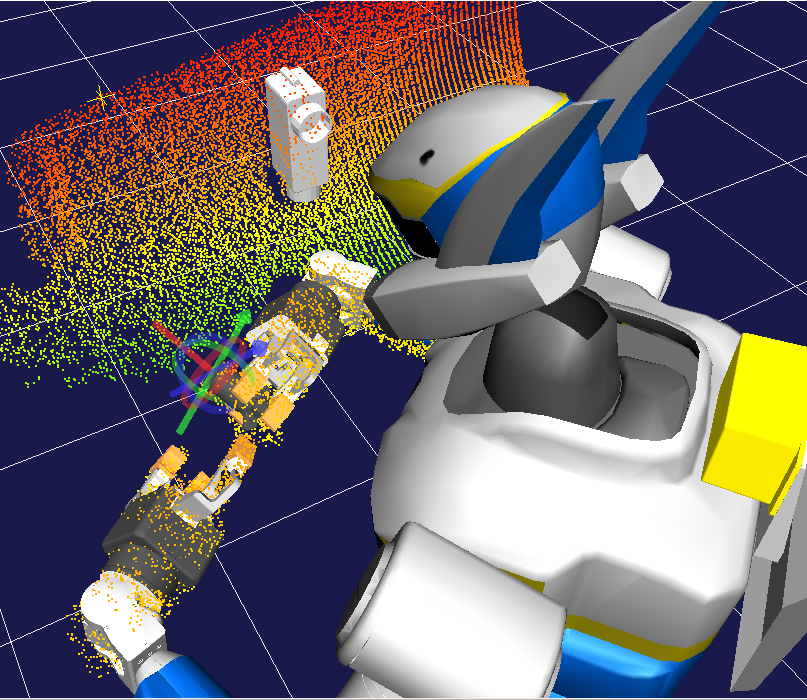
\includegraphics[height = 5cm]{img/WatchPlug}
			\caption{After pulling the plug its attitude is adjusted.}
			\label{fig:WatchPlug}
		\end{figure}
		
	\subsection{Inserting the plug}
		
		Once the Manipulation Marker representing the plug is fixed at the hand, it can further be properly
		aligned with the destination socket.
		This one can be represented with another marker (Object Marker), which can be adjusted within the
		point cloud before taking the plug to the pre-insertion position.
		However, because of inaccuracies of the point cloud, the camera at the other hand is used once again
		together with the camera at the head to look at the plug, and use this visual feedback to adjust its
		position to properly insert the plug within few movements.
		This is represented in \figurename~\ref{fig:InsertPlug}.
		
		\begin{figure}[b]
			\centering
			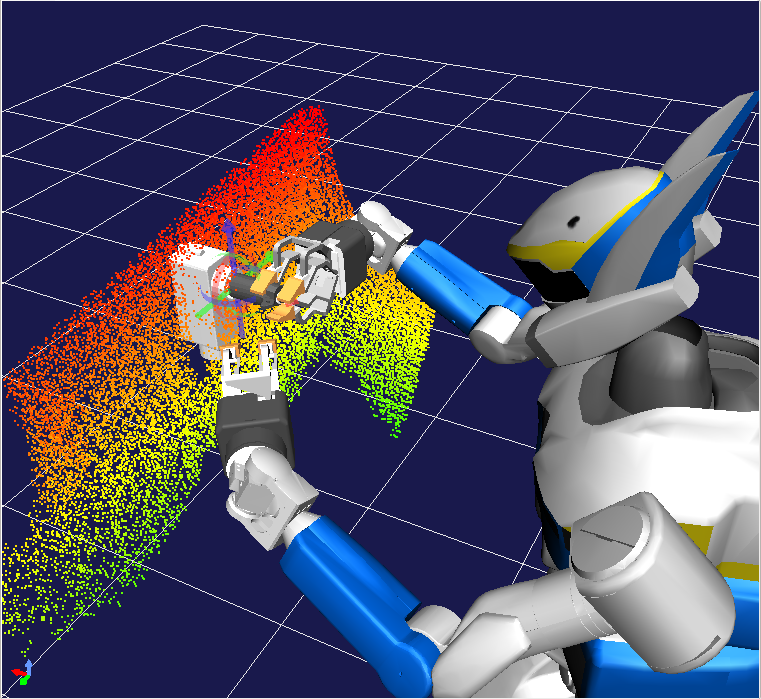
\includegraphics[height = 5cm]{img/InsertPlug}
			\caption{The plug is inserted by using visual feedback.}
			\label{fig:InsertPlug}
		\end{figure}
		
		Then, once the task is completed, the hand opens and an updated point cloud is taken, in order to
		correctly plan the returning motion without hitting the cable of the plug.
	
	%\section{Opening a box and pressing a button}
	\label{sub:button}
	
	\section{Conclusions}
	\label{sec:conclusions}
	
	The task-level teleoperation strategy presented in this paper was successfully applied
	to the HRP-2Kai humanoid robot, which was able to carry out all the manipulation tasks
	proposed for the DRC, even though there was no accurate model of the environment.
	Our principal restriction was the time limit, considering that most of the time spent
	during the task was the one required by the manual identification of the objects in the
	environment and by the verification of the robot motion by the operator.

	For the door task, we required manual positioning the door lever and grasp position alignment.
	To realize faster door passing through, those operations must be automated.

	With respect to the plug task it is worth to notice that even though its execution
	lasted 16:34 minutes, the effective time was just 1:34 and the number of adjustments
	required to insert the plug was only 3.
	This was the result of assuring a stable grasp of the plug, as well as the use of markers
	to identify the plug and the sockets.
	
	As a future work we want to improve our recognition system, in order to speed up the execution
	of every task.
	
	\bibliographystyle{unsrt}
	\bibliography{ManipulationDARPA}
	
\end{document}